\section{Envisioned final product}
A lot to be critical about this design, e.g. it doesn't really account for how braille is read and the convenience of keeping one's fingers in place. It is essentially a braille version of a sighted product.
\begin{figure}[h]
\centering
    \includegraphics[width=0.3\textwidth]{figures/e-reader.png}
\caption{}
\label{fig:e-reader.png}
\end{figure}
\section{Encoding}
Figure \ref{fig:encoding.png} describes the initial approach to convert text into braille given a device with 16 addressable cells.
\begin{figure}[h]
\centering
    \includegraphics[height=5cm]{figures/encoding.png}
\caption{Early idea for serial encoding of up to 16 braille cells.}
\label{fig:encoding.png}
\end{figure}

\section{Addressable cell}
Use of a typing element similar to IBM Selectric typewriter as shown in figure \ref{fig:IBM_Selectric_Globe_Wiki.jpg}. Viable for a printer, however the moving mechanism is too large to be embedded into a tablet-sized device. Hybrid addressable cell attempts to tackle the size issue.
\begin{figure}[h]
\centering
    \includegraphics[height=5cm]{figures/IBM_Selectric_Globe_Wiki.jpg}
\caption{IBM Selectric typing element \cite{wiki:IBMSelectric}.}
\label{fig:IBM_Selectric_Globe_Wiki.jpg}
\end{figure}

\section{Hybrid addressable cell}
As shown in figure \ref{fig:rotation.png} the characters fall partially into a slot, which means they are depressed on the surface. Each rotating disk is a saggital half of the braille cell, i.e. two disks form one braille cell.

Requires the production of either two distinct rotating disks or a spacer between each pair of disks. Unclear how the characters are able to leave the slot once depressed.
\begin{figure}[h]
\centering
    \includegraphics[width=0.6\textwidth]{figures/rotation.png}
\caption{}
\label{fig:rotation.png}
\end{figure}

\section{Individually addressable characters}
\subsection{Electromechanical}
This includes piezoelectric and the linear actuators. Not considered due to size. Examples will be addressed in the status quo analysis.

\subsection{Pneumatic}
Usage similar to \cite{XieZhixin2021A2rB}. Use of a compliant mechanism for a bi-stable switch of the character.  
\begin{figure}[h]
\centering
    \includegraphics[height=5cm]{figures/pneumatic.png}
\caption{Pneumatic actuation mechanism}
\label{fig:pneumatic.png}
\end{figure}

\subsection{Magnetic}

Linear motion electromagnetic actuator as seen in figure \ref{fig:magnet-cross_section.png}.
It consists of a variable magnet at the base that pushes a permanent magnet attached to the character. Its largest problem is size, which is briefly discussed by \cite{BettelaniGemmaCarolina2020DaVo}.


Overcoming the need for a continuous magnetic field that pushes a character up has been partially solved by the usage of a latch \cite{KimJoonyeong2020BDfP}. Results are questionable, and we end up with a design that is very similar to the pneumatic with a compliant mechanism.


\begin{figure}[h]
\centering
    \includegraphics[height=5cm]{figures/magnet-cross_section.png}
\caption{Cross-section of magnetic actuator}
\label{fig:magnet-cross_section.png}
\end{figure}


